\documentclass[11pt]{article}
\usepackage{amsmath, amssymb}
\usepackage[x12names, rgb, html]{xcolor}

\definecolor{red}{HTML}{f54b1a}
\definecolor{pink}{HTML}{d19eb1}
\definecolor{orange}{HTML}{d3772e}
\definecolor{yellow}{HTML}{ebe85d}
\definecolor{green}{HTML}{0f6852}
\definecolor{lightblue}{HTML}{01abe9}
\definecolor{darkblue}{HTML}{1b346c}
\definecolor{tan}{HTML}{e5c39e}
\definecolor{darktan}{HTML}{af9e73}
\definecolor{grey}{HTML}{c3ced0}
\definecolor{darkgrey}{HTML}{9dadc4}
\definecolor{black}{HTML}{110d1b}
\definecolor{white}{HTML}{f1f8f1}


\usepackage{hyperref}
\hypersetup{
  colorlinks = true,
  linkcolor = red,
  citecolor = darkblue,
  urlcolor = lightblue
}

\usepackage[margin=1in]{geometry}

\newcommand{\grant}[1]{\marginpar{\huge \textcolor{green}{$\star$}} \textcolor{green}{GMR: #1}}
\renewcommand{\thefootnote}{$\star$}

%\usepackage{ebgaramond}
%\usepackage[cmintegrals,cmbraces]{newtxmath}
%\usepackage{ebgaramond-maths}
% \usepackage{fontspec}
% \setmainfont[]{ebgaramond}
% \setmainfont[
%     Path = theme/,
%     Ligatures=TeX,
%     UprightFont = et-book-roman-old-style-figures,
%     ItalicFont = et-book-display-italic-old-style-figures,
%     BoldItalicFont = et-book-semi-bold-old-style-figures,
%     BoldFont = et-book-bold-line-figures
%   ]{}

\usepackage{graphicx}



\newcommand{\diff}[3]{\frac{\partial^{#3}#1}{\partial #2^{#3}}}
\newcommand{\Diff}[3]{\frac{d^{#3}#1}{d #2^{#3}}}

\newcommand{\bfm}[1]{\mathchoice {\mbox{\boldmath$\displaystyle#1$}}
    {\mbox{\boldmath$\textstyle#1$}}
    {\mbox{\boldmath$\scriptstyle#1$}}
    {\mbox{\boldmath$\scriptscriptstyle#1$}}}


\def\rhoeq{\varrho_{\rm eq}}
\def\nb{\boldsymbol{n}}
\def\rhob{\boldsymbol{\rho}}
\def\varrhob{\boldsymbol{\varrho}}
\def\thetab{\boldsymbol{\theta}}
\def\varthetab{\boldsymbol{\vartheta}}
\def\etab{\boldsymbol{\eta}}
\def\xib{\boldsymbol{\xi}}
\def\ab{\boldsymbol{a}}
\def\bb{\boldsymbol{b}}
\def\cb{\boldsymbol{c}}
\def\qb{\boldsymbol{q}}
\def\pb{\boldsymbol{p}}
\def\Qb{\boldsymbol{Q}}
\def\Jb{\boldsymbol{J}}
\def\kb{\boldsymbol{k}}
\def\rb{\boldsymbol{r}}
\def\vb{\boldsymbol{v}}
\def\wb{\boldsymbol{w}}
\def\xb{\boldsymbol{x}}
\def\yb{\boldsymbol{y}}
\def\zb{\boldsymbol{z}}

\def\Mb{\boldsymbol{M}}
\def\Tb{\boldsymbol{T}}
\def\Xb{\boldsymbol{X}}
\def\Xbu{\boldsymbol{X}^{u}}
\def\Wb{\boldsymbol{W}}

\def\Xu{X^{u}}

\def\grad{\nabla}
\def\div{\nabla \cdot}
\def\lap{\Delta}

\def\d{\displaystyle} \def\t{\textstyle} \def\scr{\scriptstyle}
\def\sscr{\scriptscriptstyle} \def\sp{\vspace{2mm}}

\def\lap{\Delta}
\def\eps{\varepsilon}

\def\RR{\mathbb{R}} \def\NN{\mathbb{N}} \def\ZZ{\mathbb{Z}}
\def\EE{\mathbb{E}}\def\PP{\mathbb{P}}

\newcommand{\ddt}{\frac{\partial}{\partial t}}
\newcommand{\ddx}{\frac{\partial}{\partial x}}
\newcommand{\avg}[1]{\left\langle #1 \right\rangle}

\def\<{\langle} \def\>{\rangle}

\DeclareRobustCommand{\ran}{\operatorname*{ran}}
\DeclareRobustCommand{\supp}{\operatorname*{supp}}
\DeclareRobustCommand{\argmin}{\operatorname*{argmin}}
\DeclareRobustCommand{\sign}{\operatorname*{sign}}


\title{Sampling thermodynamic ensembles of molecular systems with generative neural networks: Will integrating physics-based models close the generalization gap?}
\author{Grant M. Rotskoff}
\date{\today}

\usepackage{fancyhdr}

\fancypagestyle{fancy}{%
\fancyhf{}% clear all header and footer fields
\renewcommand{\headrulewidth}{0pt}%
\renewcommand{\footrulewidth}{0pt}%
}

\fancypagestyle{plain}{%
\fancyhf{}% clear all header and footer fields
\fancyfoot[L]{\textcolor{darkblue}{Last $\Delta$ = \today}} % except the center
\renewcommand{\headrulewidth}{0pt}%
\renewcommand{\footrulewidth}{0pt}%
}

%\graphicspath{figures}


\begin{document}

\maketitle

\begin{abstract}
If the promise of generative modeling techniques is realized, it may fundamentally change how we carry out molecular simulation.
The suite of techniques and models collectively termed ``generative AI'' includes many different classes of models, built for varied types of data, from natural language to images.
Recent advances in the machine learning literature that construct ever better generative models, though, do not contend with the challenges unique to complex, molecular systems. 
To generate a statistically likely molecular configuration, many correlated degrees of freedom must be sampled together, while also satisfying the strong constraints of chemical physics. 
Recent efforts to develop generative models for biomolecular systems have shown spectacular results in some cases---nevertheless, some simple systems remain out of reach with our present methodology.
Arguably, the central concern is data-efficiency: we should aim to train models that can meaningfully generalize beyond their training data and hence facilitate discovery.
In this review we discuss methods and future directions for directly incorporating physics-based models into generative neural networks, which we believe is a crucial step for addressing the limitations of the current toolkit.
\end{abstract}



% %% use optional labels to link authors explicitly to addresses:
% \author[label1,label2]{Grant M. Rotskoff}
% \affiliation[label1]{organization={Department of Chemistry, Stanford University},
%             %addressline={Keck Science Building},
%             city={Stanford},
%             postcode={94305},
%             state={CA},
%             country={USA}}
% %%
% \affiliation[label2]{organization={Institute for Computational and Mathematical Engineering},
%             %addressline={},
%             city={Stanford},
%             postcode={94305},
%             state={CA},
%             country={USA}}

% % \affiliation{organization={Stanford University},%Department and Organization
% %             addressline={}, 
% %             city={},
% %             postcode={}, 
% %             state={},
% %             country={}}


%% main text
\section{Introduction and background}
\label{sec:intro}


Supervised machine learning has a rich history in the chemical sciences~\cite{lederberg_applications_1969}. 
For many decades, fitting linear and nonlinear regression models to experimental data has been a central modality of data-driven science.
In the last decade, both the complexity and expressiveness of the available models have grown rapidly: as the library of neural network architectures expanded, models that are well-calibrated for chemical and dynamical data have been widely and enthusiastically deployed in experimental and theoretical chemistry~\cite{mater_deep_2019}. 
While these algorithmic innovations have spurred substantive progress in chem-informatics~\cite{mater_deep_2019} and the physical sciences more broadly~\cite{carleo_machine_2019}, one cannot discount the formative role played by increasingly powerful computational resources~\cite{amodei_ai_2018} alongside sophisticated and reliable software for automatic differentiation and optimization~\cite{paszke_pytorch_2019, bradbury_jax_2018, broughton_tensorflow_2020}. 
Together, these developments have led to an active community of research designing ever better networks, optimization strategies, and data curation to further improve the performance of data driven models.

A comparably new modeling paradigm is emerging alongside the developments in supervised learning due to the extraordinary developments in generative modeling.
Often called ``unsupervised learning'' as a contrast with regression or classification tasks on labelled data, generative models seek to directly emulate data.
For the purposes of this review, we will define a generative model to be any model that is parameterized to draw samples from a target probability distribution.
Information about a target probability distribution is either accessible through a data set of samples drawn from the distribution or, alternatively, through the unnormalized statistical likelihood function, which for a Gibbs-Boltzmann distribution is simply the energy.  
Generative models have attracted enormous attention for applications outside of science, such as text-to-image generation with denoising diffusion models~\cite{song_score-based_2022,ho_denoising_nodate} and auto-regressive text generation with large language models (LLMs)~\cite{vaswani_attention_2017}. 
The natural question, of course, is whether or not these approaches can amplify and accelerate scientific inquiry in the chemical context.

In this review, we seek to articulate the potentialities and challenges of using generative models to sample finite temperature equilibrium probability distributions of chemical systems in the condensed phase.
We emphasize that this task is considerably different from, for example, protein structure prediction using alphaFold~\cite{jumper_highly_2021}, which predicts the crystal structure but does not capture molecular fluctuations.
Perhaps the defining challenge facing the generative modeling paradigm is \emph{generalization}: in many complex scientific tasks, large repositories of training data simply do not exist and generative models must instead be built from smaller data sets than those used for image generation applications or LLMs; in the latter case, empirical scaling laws show that increasing amounts of data improve the test loss as a power law~\cite{kaplan_scaling_2020, dyer_explaining_2021}.
If a generative model can only effectively sample molecular configurations that are very close to those provided in an initial data set, then little useful information can be gained from sampling the generative model. 
Nevertheless, researchers are actively building strategies to augment data, improve transferability, and enhance generalization by integrating generative models into enhanced sampling schemes already widely used in molecular simulation.

To provide a comprehensive overview of the challenges and opportunities afforded by generative models, we will first review current modeling paradigms, neural network architectures, and training approaches, without specializing to molecular systems. 
We will then discuss efforts to incorporate \emph{physical inductive bias}, that is, natural physical invariance and equivariance into generative neural networks, which promises to improve the quality of the generated samples and reduce training effort.
Our central focus will be on the question generalization and we will discuss several distinct strategies that seek to improve the capacity of these models for discovery, a question that remains formative for this new and developing field.


\section{Generative modeling for molecular systems}

For a molecular system in thermal equilibrium at constant temperature, volume, and particle number, we know from elementary statistical mechanics~\cite{chandler_introduction_1987} that the probability density of a given configuration can be written as,
\begin{equation}
    \rhoeq(\xb) = Z^{-1} e^{-\beta U(\xb)},
    \label{eq:rhoeq}
\end{equation}
where $\beta=1/(k_{\rm B} T)$, $U$ is the potential energy function for the system, and $Z = \int_{\Omega} e^{-\beta U(\xb)} d\xb$ is the normalization constant for the distribution, also called the partition function. 
Of course, it is not possible to evaluate $\rhoeq$ directly because the partition function is ``intractable'', requiring that we compute a high-dimensional integral which is typically impossible.

Because we have accurate models of the energy $U$ from either electronic structure methods or classical approximations collectively referred to as molecular force fields~\cite{case_amber_2005, vanommeslaeghe_charmm_2010}, we usually draw samples from~\eqref{eq:rhoeq} with Markov chain Monte Carlo (MCMC) sampling algorithms.
Access to a collection of configurations allows us to estimate observable properties of the system by evaluating an ``empirical expectation'' or sample average,
\begin{equation}
\begin{aligned}
    \avg{\mathcal{A}} &= Z^{-1} \int_{\Omega} \mathcal{A}(\xb) e^{-\beta U(\xb)} d\xb, \\
    &\approx \frac1n \sum_{i=1}^n \mathcal{A}(\xb_i), \quad \xb_i \sim \rhoeq,
    \label{eq:avg}
\end{aligned}
\end{equation}
for any observable function $\mathcal{A}.$
In principle, estimating \eqref{eq:avg} is straightforward, requiring only a direct MCMC simulation or a molecular dynamics (MD) simulation in which the samples have been appropriately ``metropolized'' to ensure Boltzmann statistics~\cite{frenkel_understanding_2002}. 
In practice, such estimates rarely converge quickly because molecular systems often have metastable probability distributions, as illustrated in Fig.~\ref{fig:metastable}. 
The amount simulation time and hence computational effort required for MD or MCMC to ``mix'' between the two metastable configurations is simply prohibitive in many processes of interest~\cite{lelievre_free_2010}.

Generative models, which seek to directly approximate $\rhoeq$ and sample efficiently from it, do not suffer from the issue of slow mixing because each new sample is statistically uncorrelated from the last.
However, we must optimize a parametric model to approximate the target probability distribution, which itself incurs a computational cost.
Supposing that we build a generative model with parameters $\theta$ for which we can compute exactly the normalized probability density of the samples we generate $\rho_{\theta}$, then the associated Metropolis-Hastings acceptance criterion a newly proposed configuration in a Markov chain $\xb_0, \dots, \xb_k$ is~\cite{gabrie_adaptive_2022},
\begin{equation}
    \textrm{acc}(\xb_k \to \xb_{k+1}) = \min \left[ 1, \frac{\rhoeq(\xb_{k+1})\rho_{\theta}(\xb_{k}) }{\rhoeq(\xb_{k})\rho_{\theta}(\xb_{k+1}) }\right].
\end{equation}
Importantly, this scheme correctly accounts for the proposal distribution and has the transparent outcome that, if the generative model is identical to the Boltzmann distribution, the acceptance probability is unity. 
This discussion assumes, of course, that it is possible to efficiently build a generative model that i) accurately approximates a given target distribution and ii) allows accurate or exact evaluation of $\rho_{\theta}$ for an arbitrary sample. 
Neither of these assumptions should be taken for granted: we will focus primarily on these questions in the present review.


In general, there are two distinct strategies for building a generative model to represent a Boltzmann distribution: \emph{training with data} and \emph{training with energy}, which we discuss in detail below. 

\begin{figure*}
\begin{center}
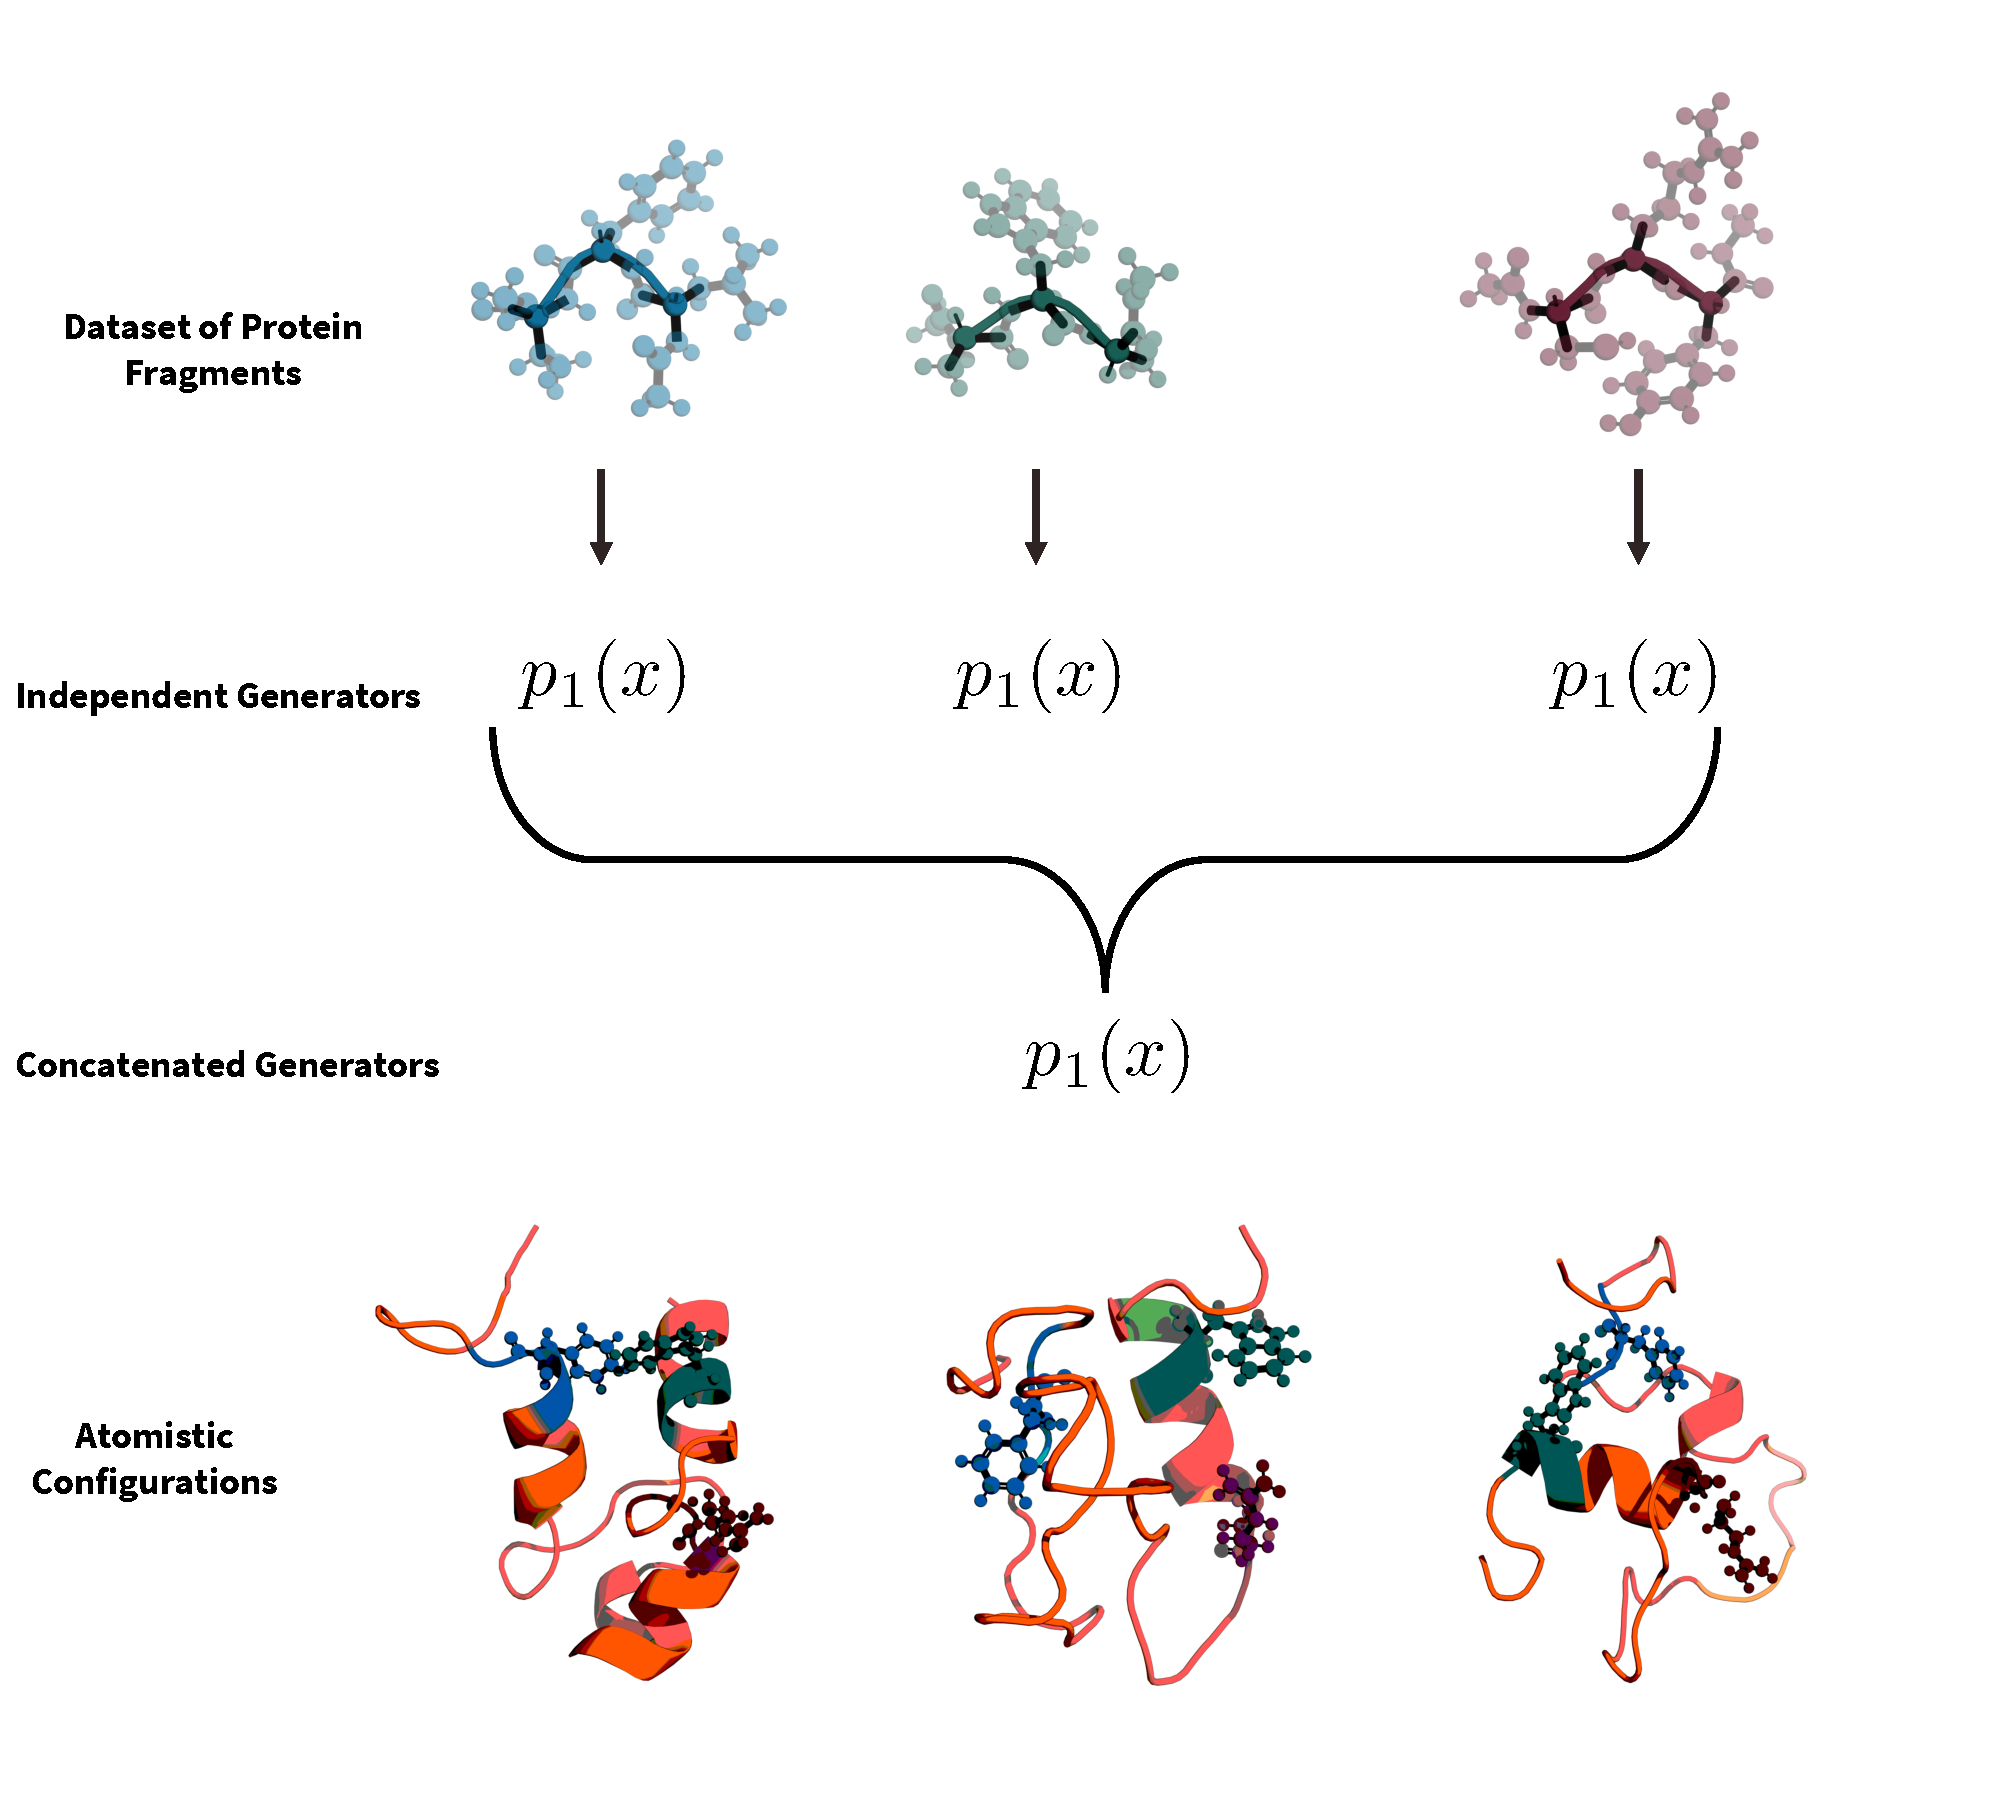
\includegraphics[width=0.5\linewidth]{modular_fig.pdf}
\end{center}
\caption{Schematic overview of different types of models under consideration. (a) Denoising diffusion models. (b) Continuous normalizing flows and flow-matching models. (c) Normalizing flows based on coupling layers and compositional invertible maps.}
\label{fig:models}
\end{figure*}

\subsection{Models trained purely with data}

The most widely used strategies for building generative models require training data.
In some sense, when training with data, these problems become supervised learning problems in which a probabilistic model is trained to recapitulate the data and smoothness is exploited to obtain ``nearby'' configurations.
Many modern generative neural networks were designed for image data, where, as we can intuitively recognize, small perturbations do not typically affect our ability to interpret the result. 
However, this is not the case for molecular systems: a single particle-particle overlap or a violation of chemical bonding rules can be catastrophic. 

In the following discussion, we will focus on two closely related generative modeling strategies, namely, denoising diffusion probabilistic models, which we will simply call \emph{diffusion models}, and flow matching models~\cite{lipman_flow_2022, albergo_building_2022, albergo_stochastic_2023} which are also known as stochastic interpolants.  
There are many classes of generative models that we choose not to discuss here, including generative adversarial networks~\cite{goodfellow_generative_2014} and restricted Boltzmann machines~\cite{salakhutdinov_restricted_2007, salakhutdinov_deep_2009} because, while powerful, these models are lesser used in the applications of interest to this review. 

When discussing models trained with data, we will assume that we are given a data set consisting of $n$ points, denoted $\mathcal{D} = \{ \xb_i \}_{i=1}^n$.
While the frameworks are far more general, the applications we have in mind are those for which each point $\xb_i$ is a molecular configuration and is distributed according to a Boltzmann distribution, i.e., $\xb_i \sim \rhoeq.$

\subsubsection{Denoising diffusion models}

Diffusion models were initially developed in Ref.~\cite{sohl-dickstein_hamiltonian_2012} using a theoretical framework built from ideas about time-reversed dynamics originally in the nonequilibrium statistical mechanics literature~\cite{crooks_entropy_1999, kurchan_fluctuation_1998, lebowitz_gallavotticohen-type_1999}. 
At a high level, the idea of diffusion models to define a stochastic process in which we progressively transform samples from a data set into statistical noise.
Among the mostly widely used approaches is to simulate an Ornstein-Uhlenbeck process starting from a data point $\xb$.
Explicitly, for some time interval $[0, T]$, we use
\begin{equation}
    d\Xb_t = - g(t) \Xb_t dt + \sqrt{2 g(t)} d\Wb_t; \quad \Xb_0 = \xb.
    \label{eq:ou}
\end{equation}
Because an Ornstein-Uhlenbeck process converges exponentially fast to Gaussian distribution, for sufficiently large times $T$, the samples are nearly indistinguishable from Gaussian random variables. 

The key insight underlying diffusion models is that, with the collection of trajectories obtained by the noising dynamics~\eqref{eq:ou}, we can learn a representation of the time-reversal of this dynamics and convert noise into samples that resemble the target distribution.
In fact, Fokker-Planck equation associated with the stochastic process defined in~\eqref{eq:ou} has an exact time-reversal~\cite{anderson_reverse-time_1982,song_score-based_2022} which leads to the unknown reverse process,
\begin{equation}
    d\tilde{\Xb}_t = -g(t)[\tilde{\Xb}_t + \nabla \log \rho_t(\tilde{\Xb}_t)] dt + \sqrt{2 g(t)} d\tilde{\Wb}_t; \quad \tilde{\Xb}_0\sim \mathcal{N}(0,\rm{Id}).
    \label{eq:revou}
\end{equation}
A generative model is constructed by approximating the ``score'' of the intermediate time distributions, $\nabla \log \rho_t$, using a neural network $s(\xb, t; \theta)$.
This procedure is known as score-matching~\cite{song_score-based_2022} and a converged score function enables sampling from the data distribution simply by simulating~\eqref{eq:revou}.
To optimize the score, we minimize an objective~\cite{song_score-based_2022} in which the conditional score appears explicitly,
\begin{equation}
    \mathcal{L}_{\rm score}(\theta) = \EE_t \EE_{\xb_t| \xb_0, \xb_0} \left\| s_{\theta}(\xb_t, t) - \nabla \log \rho_t (\xb_t | \xb_0) \right\|^2,
\end{equation}
where the expectations here are computed uniformly in time $t$, with $\xb_0 \sim \rho_0$, and $\xb_t$ sampled from the distribution of stochastic trajectories starting from $\xb_0$ at time $t=0.$
Knowledge of the conditional score enables regression, but an explicit expression for $\log \rho_t (\cdot | \xb_0)$ is only available when the noising SDE is linear, and hence the conditional distribution at intermediate times is Gaussian.
This poses, at the very least, an obstacle to making a physics-informed choice of the noising SDE. 
Diffusion models have already been embraced in a variety of contexts, and while there are several different formalisms (discrete time~\cite{ho_denoising_nodate}, continuous time~\cite{song_score-based_2022,vroylandt_likelihood-based_2022}) all these approaches share in common a dynamics that flows samples from a data set to a tractable distribution and a data-dependent parameterization of the inverse dynamics.
%See ~\cite{} for a comprehensive overview. 

Diffusion models have a variety of advantages that make them suitable for working with physical systems. 
One important aspect of the generative process is that the physical invariants can be directly incorporated into the score function.
For example, ~\cite{schneuing_structure-based_2022,weiss_guided_2023} introduced parameterizations of the score that are equivariant with respect to rotations, translations invariant, and permutation invariant for identical atoms.
Ensuring that physical invariances are respected is believed to aid data-efficiency and improve generalization, and there is some empirical evidence to support this belief~\cite{sannai_improved_2021}.
Furthermore, it is possible incorporate physics-based regularizations~\cite{zheng_towards_2023}, which could be useful for treating systems with hard-core repulsive interactions or long-ranged Coulombic interactions.

Ensuring detailed balance within a Metropolis-Hastings scheme requires accounting for asymmetry in the proposal distribution~\cite{frenkel_understanding_2002}.
For generative models, this means that the acceptance criterion for an MCMC proposal is simply
\begin{equation}
    \textrm{acc}(\xb_{k} \to \xb_{k+1}) = \min \left[ 1, \frac{\hat{\rho}(\xb_{k})}{\hat{\rho}(\xb_{k+1})} e^{-\beta \Delta U(\xb_{k+1},\xb_k)} \right].
    \label{eq:mhacc}
\end{equation}
Because the normalization constant cancels in the ratio of generative model probabilities in \eqref{eq:mhacc}, we need only the unnormalized statistical weights associated with the samples, typically called the likelihood in the Bayesian context.
While it is possible to compute exact likelihoods by solving a probability flow ODE, 
\begin{equation}
    \log \hat\rho(\xb_0) = \log \hat\rho(\xb_T) - \int_0^T g(t) \bigl( d + \nabla \cdot s_{\theta}(\xb_t,t) \bigr) dt,
    \label{eq:pfode}
\end{equation}
where $d$ is the dimensionality.
This equation can be difficult to employ in practice because integrating the divergence is computationally expensive and approximating the trace of the gradient is often the only option~\cite{grathwohl_ffjord_2018}. 

\begin{figure*}
    \centering
    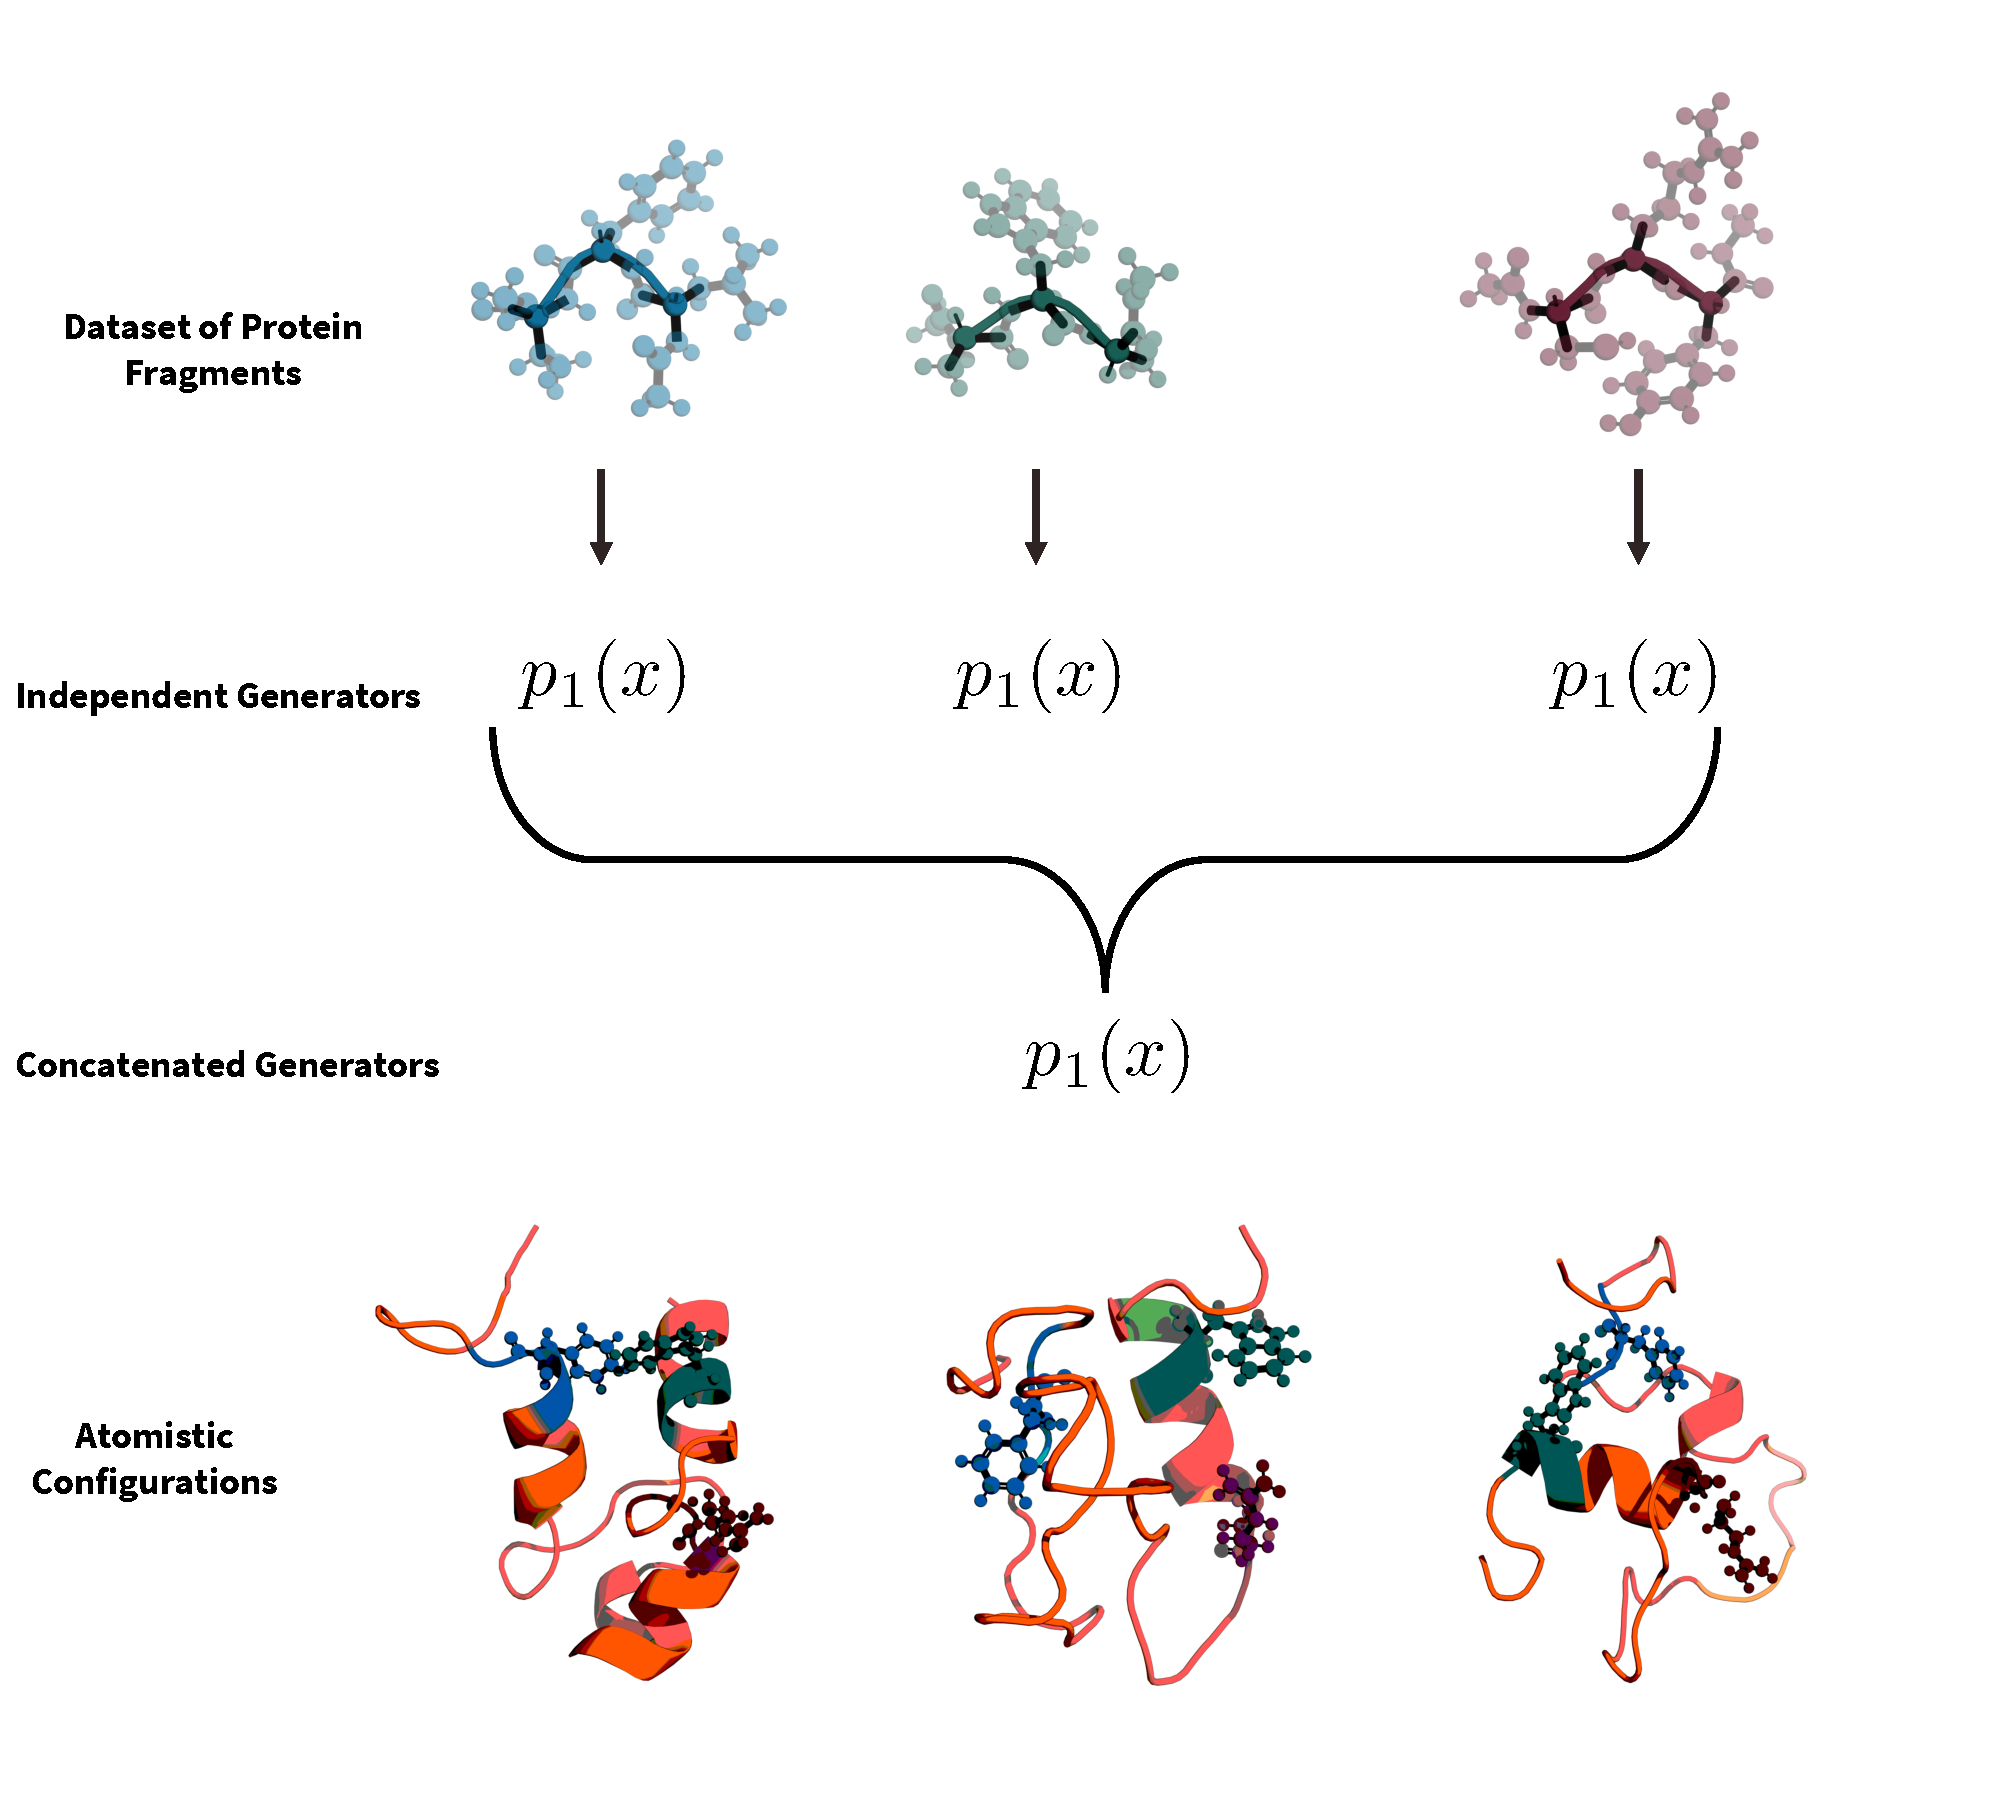
\includegraphics[width=0.6\linewidth]{modular_fig.pdf}
    \caption{Caption}
    \label{fig:enter-label}
\end{figure*}

\subsubsection{Flow-based models}

The idea of transforming samples from an ``easy'' distribution, like a Gaussian, into intricately structured random variables has also motivated more direct approaches.
Normalizing flows~\cite{tabak_density_2010,rezende_variational_2015} seek to transform a tractable initial distribution into samples with high probability in the target distribution with a single map.
Such a transformation, which depends on optimizable parameters $\theta$ and we denote $T_{\theta}$, generates samples by ``pushing forward'' samples from the initial distribution. 
Importantly, normalizing flows are chosen to be invertible functions, meaning that the probability of samples generated by transforming noise with $T_{\theta}$ can be evaluated exactly.
Explicitly,
\begin{equation}
\begin{aligned}
    \xb &= T_{\theta}(\zb) \quad \zb \sim \rho_0, \\
    \hat \rho_\theta(\xb) &= \rho_0(T_{\theta}^{-1}(\xb)) |\nabla T_{\theta}^{-1}(\xb)|,
\end{aligned}
\end{equation}
where $\rho_0$ is the tractable initial distribution and the notation $|\nabla f|$ denotes the determinant of the Jacobian, which arises simply from change of variables. 
Among the most widely used normalizing flow architectures are RealNVP coupling layers~\cite{dinh_density_2017} and rational quadratic splines~\cite{}.
The requirement of invertibility is a strong constraint and the currently available normalizing flow models can be challenging to optimize~\cite{}.

An alternative strategy for building invertible maps exploits the \emph{neural ordinary differential equations}~\cite{chen_neural_2018} framework.
The free-form Jacobian of continuous dynamics (FFJORD) algorithm exploits the classical adjoint state method to optimize an parametric ordinary differential equation using a maximum likelihood loss function. 
In some examples, normalizing flows built with continuous-time ODEs add significant flexibility to models compared with those built on coupling layers which have a restricted functional form.
This approach is, however, limited computationally due to the requirement that the ODE be solved numerically for sample generation. 
Furthermore, computing exact likelihoods is not tractable for high-dimensional systems because the trace of the Jacobian matrix requires $\mathcal{O}(d^2)$ operations in dimension $d$ at every step of the ODE solve.
To mitigate this, the trace is typically estimated using the Hutchinson trace estimator~\cite{hutchinson_stochastic_1989}, but the variance can be problematic in practice. 

Recent works that seek to extend and enhance the framework of continuous normalizing flows have introduced flow matching~\cite{peluchetti_non-denoising_2022,peluchetti_diffusion_2023,lipman_flow_2022} or stochastic interpolants~\cite{albergo_building_2022, albergo_stochastic_2023}.
A representation of the direct transformation between two distributions is parameterized using only a vector field $v_{\theta}: \RR^d\times[0,1]\to \RR^d$ and samples from the target distribution $\rho_1$ are obtained by solving the initial value ODE,
\begin{equation}
    \dot \xb_t = v_{\theta}(\xb,t), \quad \xb_0 \sim \rho_0.
\end{equation}
In this generative modeling framework, the transformation between the tractable Gaussian distribution and the target is first built sequence of simple intermediate distributions for which the associated flow field can be specified by linear interpolants~\cite{lipman_flow_2022, albergo_building_2022}, 
\begin{equation}
    I(x_0, x_1, t) = \alpha(t) x_0 + \beta(t) x_1 + \gamma(t) z,
\end{equation}
where $\alpha(0)=1$ and $\beta(0)=0$, $\alpha(1)=0$ and $\beta(1)=1$.
The interpolating function can be made noisy by choosing a non-zero function $\gamma(t)$ such that $\gamma(0)=0$ and $\gamma(1)=0$ and $z$ is a Gaussian random variable.
The time derivative of the interpolant $I$ provides a ``flow-matching'' objective
\begin{equation}
    \mathcal{L}_{\rm FM} = \EE_{t} \EE_{\xb_0, \xb_1} \| v_\theta(\xb, t) - \dot I(\xb_0, \xb_1, t) \|^2.
\end{equation}
These expectations can be evaluated explicitly using a data set and samples from the easily sampled distribution $\rho_0$.

These models share many commonalities with diffusion models, but differ in several potentially important ways.
For diffusion models, the noising dynamics~\eqref{eq:ou} does not completely lose memory of its initial condition in a finite time, meaning that the noise samples are not exactly Gaussian distributed, though there have been recent efforts to ameliorate this problem~\cite{shi_diffusion_2023}.
Because flow-matching models learn a transformation directly between a noise distribution and the target distribution, no approximation is needed to use these models as generative models. 
Furthermore, the relatively implicit objective function used in score-matching constrains choice the noising dynamics: it will be computationally efficient only if~\eqref{eq:ou} is linear.
Flow-matching models, on the other hand, are optimized using regression directly on the learned velocity field. 
For modeling physical systems, this means that natural regularization terms and constraints can be directly incorporated into the entire generative process. 
While these models have not yet been used widely for physical data, these properties suggest that they could provide a productive avenue for sampling molecular systems. 
However, like diffusion models, likelihood estimation is difficult. 
Computing the likelihood of samples generated from the learned velocity field requires an integral analogous to \eqref{eq:pfode} which will not be tractable in high-dimensional systems.


\subsubsection{Generic challenges with data-based training}

Both diffusion models and flow-based models are trained purely with data, which means that we have not exploited knowledge of the statistical likelihood---i.e., the energy---at all. 
While we can only speculate at this point, we believe that training with the energy function will provide much needed information in cases where the energy is \emph{rugged}.
Some recent theoretical work has established that inference using diffusion models is statistically \emph{hard} for high-dimensional spin glass models~\cite{ghio_sampling_2023}, but it is not clear whether explicitly incorporating information from the model, or alternatively using an adaptive Monte Carlo strategy~\cite{gabrie_efficient_2021, gabrie_adaptive_2022} would improve the performance.
Furthermore, data-based generative models are not manifestly useful for the physical sciences unless they can meaningfully generalize to samples far from the training set; it is unclear at present how much data might be necessary for physical systems to achieve good generalization.


\subsection{Models trained with statistical likelihoods} \label{sec:nfs}

Because computing statistical likelihoods is straightforward by construction for normalizing flow models, it is also possible to use a maximum likelihood approach to train the model. 
To do, we use the ``forward'' KL divergence as the loss function
\begin{equation}
\begin{aligned}
    D_{\rm KL}(\hat\rho_{\theta} \| \rhoeq) &= \int \log \frac{\hat\rho_{\theta}(\xb)}{\rhoeq(\xb)} \hat\rho_{\theta}(\xb) d\xb \\
    &= \EE_{\hat\rho_\theta} \left( \log \hat\rho_{\theta} + \beta U(\xb) \right)
    \label{eq:energy_kl}
\end{aligned}
\end{equation}
The appeal of this training modality is that it requires, in principle, \emph{no data}.
The samples are generated by pushing forward random variables from the tractable base distribution $\rho_0$ with the parametric map $T_{\theta}$.
In the context of thermal physical systems, the configurations are Boltzmann distributed, and the statistical likelihood is the unitless temperature-scaled energy $-\beta U.$
For this reason, we also refer to this training procedure as \textit{energy based} training.

Unfortunately, the objective \eqref{eq:energy_kl} fails in practice due to a phenomenon called \textit{mode collapse}. 
Mode collapse is characterized by the probability mass of the distribution parametrized by the normalizing flow concentrating on a single metastable state.
This phenomenon is illustrated in Fig.~\ref{fig:models} (c).
The propensity of energy based training to suffer from mode collapse can be mitigated to some extent with regularization~\cite{deldebbio_efficient_2021}.
However, even systematic alterations to the loss function do not seem sufficient to avoid mode collapse, though they can mitigate the effect to some extent~\cite{felardos_designing_2023}.

A more reliable method for avoiding mode collapse is to retain probability mass in known modes during training~\cite{gabrie_adaptive_2022}.
While this strategy seems to work in general settings, it requires \emph{a priori} knowledge of the modes.
Mode discovery likely requires directly sampling from physics-based models.
Alternatively, through the means described in the following sections, it may be possible to augment generative models with physical models for mode discovery. 

\section{Direct density estimation with normalizing flows}

Energy-based training of generative models offers the tantilizing possibility of discovering new molecular configurations while training a model. 

- energy based training more natural, but suffers from mode collapse
- data based training more interpolative, so less to learn from the model
- Boltzmann generators were an unmitigated disaster that misled everyone and are still confusing the literature
- recent works show that augmenting with additional mcmc steps helps

Along a similar line of inquiry to Ref.~\cite{ghio_sampling_2023}, normalizing flow based MCMC strategies have been shown to fail for complex constraint satisfaction problems~\cite{ciarella_machine-learning-assisted_2023}.
However, these problems are computationally hard in the

\subsection{Adapting normalizing flow models for physical systems}

While it was apparent that normalizing flows could be used a transition density (also called generation probabilities) in a Markov chain Monte Carlo algorithm~\cite{rezende_variational_2015}, No\'{e} et al.~\cite{noe_boltzmann_2019} were the first to show that this approach could be used in the context of physics-based models of molecular systems like proteins.
Alternative approaches for parameterizing transition densities had also been proposed, including strategies based on Hamiltonian Monte Carlo~\cite{levy_generalizing_2018} and nonlinear independent component estimators~\cite{song_-nice-mc_2017}, but these have not been thoroughly explored for condensed phase systems like proteins. 
In Ref.~\cite{noe_boltzmann_2019}, the strategy requires a large training data for molecular systems, because a data-dependent Gaussianization, known as PCA whitening, is used to preprocess the data. 
This approach reduces the learning burden on the normalizing flow because the target distribution has been transformed to be approximately Gaussian. 

A set of subsequent investigations provided more exacting test of the statistical accuracy of sampling strategies built on density estimation with normalizing flows. 
Work by Wirnsberger and co-workers~\cite{wirnsberger_normalizing_2021, wirnsberger_estimating_2023} compared sampling with normalizing flows to the classical Frenkel Ladd thermodynamic integration approach~\cite{frenkel_new_1984}.


introduced an elegant parameterization of the a normalizing flow in which the tractable distribution was a mixture of truncated Gaussians at atom

considered instead 


- informed based measures

- permutation symmetry and periodic boundary conditions

- recent works with diffusion models integrating PINN loss terms

\section{Augmenting mode discovery with coarse-grained models}

The dual problem of mode collapse and lack of data requires fundamentally different approaches for building generative models to sample thermodynamic ensembles.
Several recent works have sought to enhance sampling by carrying out dynamics in a ``latent'' space and subsequently recovering the atomistic molecular configuration using a generative model.
Sidky et al.~\cite{sidky_molecular_2020} were among the first to use this approach which builds a generative adversarial network from molecular dynamics trajectory data. 

More recently, combining coarse-grained models with generative models has emerged as a strategy to accelerate the rate of mixing between metastable states, potentially discovering new metastable basins.
Conditional normalizing flows---less data is needed, reconstruction of Gaussian degrees of freedom
Can be trained end-to-end

Similar techniques have been proposed to bridge levels of electronic structure theory

As CG models themselves benefit from increasingly powerful supervised learning, we should remain optimistic

\section{Enhancing sampling with normalizing flows}

The strong constraints on normalizing flows limit their expressive power, but also make available some interesting algorithmic innovations:

- skipping the replica exchange ladder
- Doucet stuff
- pratyush ddpm replica exchange 

\section{Challenges and outlook}

The aim of this forward-looking review is to establish a challenge for the community working at the interface generative machine learning and physical chemistry to build models that will enable discovery rather than models that accurately reflect their training data. 
The role of strong physical inductive biases in this challenge is becoming clear: even in simple systems, state-of-the-art generative models can fail to capture the subtle correlations  


 \bibliographystyle{alpha} 
 \bibliography{references}

\end{document}